\documentclass[a4paper,11pt]{article}

\usepackage[utf8]{inputenc}
\usepackage[T1]{fontenc}
\usepackage[english]{babel}
\usepackage[margin=2.5cm]{geometry}
\usepackage{graphicx}
\usepackage{booktabs}
\usepackage{siunitx}
\usepackage{amsmath}
\usepackage{hyperref}
\usepackage{listings}
\usepackage{xcolor}
\usepackage{caption}
\usepackage{subcaption}
\usepackage[numbers]{natbib}

\graphicspath{{../figures/}}

\lstdefinestyle{python}{
    language=Python,
    basicstyle=\ttfamily\small,
    keywordstyle=\color{blue!70!black}\bfseries,
    stringstyle=\color{red!60!black},
    commentstyle=\color{green!50!black}\itshape,
    numbers=left,
    numberstyle=\tiny\color{gray},
    numbersep=8pt,
    frame=single,
    framerule=0.4pt,
    rulecolor=\color{gray!50},
    backgroundcolor=\color{gray!5},
    breaklines=true,
    showstringspaces=false,
    tabsize=4,
    xleftmargin=1.5em,
    framexleftmargin=1.5em,
    aboveskip=1em,
    belowskip=1em,
}

\lstset{style=python}

\title{%
    \textbf{Bathymetric Terrain Analysis of the Catalan Coast}\\[0.5em]
    \large Data Exploration Report\\
    \large SotaMar --- Spatial Data Infrastructure for Dive Site Cataloging
}
\author{Juan}
\date{March 2026}

\begin{document}
\maketitle

\begin{abstract}
This report documents the exploration of high-resolution (1\,m) bathymetric data from the
Institut Cartogr\`afic i Geol\`ogic de Catalunya (ICGC) for dive site terrain
characterization along the Catalan coast. We describe the data access methodology via Cloud
Optimized GeoTIFF (COG) remote reading, perform a detailed pilot analysis at the Illes
Medes Marine Protected Area, and extend the terrain analysis to six sites spanning the
full 240\,km coastline. Four morphometrics are computed at each site: slope, fine-scale and
broad-scale Bathymetric Position Index (BPI), and Vector Ruggedness Measure (VRM).
Cross-site comparison reveals that VRM is the most consistent single discriminator of
dive-relevant terrain, correctly separating geomorphologically interesting sites from
featureless shelf. A case study of El Biotop artificial reef (Torredembarra) exposes a
temporal limitation: the 22\,m-tall structure is absent from the data, indicating that
survey acquisition predates its 2023 construction.
\end{abstract}

\tableofcontents
\newpage

%=============================================================================
\section{Introduction}
\label{sec:intro}
%=============================================================================

The SotaMar project aims to build a spatial data infrastructure (SDI) for cataloging
recreational scuba dive sites along the Catalan coast, integrating bathymetric terrain
analysis with dive site metadata. Before designing the system architecture, we perform a
data exploration phase to understand the available bathymetric data and validate that
derived terrain metrics can capture dive-relevant geomorphological features.

The Illes Medes (Medes Islands) near L'Estartit were chosen as the pilot area due to their
status as a Marine Protected Area, their complex underwater topography (walls, tunnels,
pinnacles), and their importance as a dive tourism destination with approximately 80,000
dives per year \citep{lloret2008}.

%=============================================================================
\section{Data Source: ICGC Bathymetry}
\label{sec:data}
%=============================================================================

\subsection{Dataset Description}

The ICGC distributes a coastal bathymetric-topographic elevation model covering the Catalan
littoral fringe as a single Cloud Optimized GeoTIFF (COG). Table~\ref{tab:metadata}
summarizes the dataset characteristics obtained by remote inspection.

\begin{table}[ht]
\centering
\caption{ICGC bathymetry COG metadata.}
\label{tab:metadata}
\begin{tabular}{@{}ll@{}}
\toprule
Property        & Value \\
\midrule
Format          & GeoTIFF (Cloud Optimized) \\
File size       & \SI{3.3}{GB} \\
Grid dimensions & \num{238202}~$\times$~\num{223252} pixels \\
Resolution      & \SI{1}{m}~$\times$~\SI{1}{m} \\
Data type       & 32-bit float \\
CRS             & EPSG:25831 (ETRS89 / UTM zone 31N) \\
Compression     & Deflate \\
Overview levels & 9 (2$\times$ to 512$\times$) \\
NoData value    & $-9999$ \\
Vertical datum  & EGM08D595 geoid (orthometric heights) \\
Full extent (E) & \SIrange{289416}{527618}{m} \\
Full extent (N) & \SIrange{4475476}{4698728}{m} \\
\bottomrule
\end{tabular}
\end{table}

\subsection{COG URL Discovery}

The dataset URL was not documented in the ICGC's WMS GetCapabilities response or
public metadata catalogs. It was discovered by browsing the Apache directory index at
\texttt{datacloud.icgc.cat/datacloud/batimetria/tif\_unzip/}, which revealed the file:

\begin{center}
\small\texttt{batimetria-v2r1-elevacions-2021-2025.tif}
\end{center}

The inclusion of \texttt{elevacions} in the filename---absent from other ICGC product
naming patterns---was the key discovery obstacle. An automated probing script was written
to systematically try candidate URL patterns before falling back to directory listing
inspection.

\subsection{Remote COG Access}

The COG format supports HTTP range requests, allowing \texttt{rasterio} (via GDAL's
\texttt{/vsicurl/} virtual filesystem) to read arbitrary spatial subsets without
downloading the full file. The following GDAL configuration was used for optimal
performance:

\begin{lstlisting}
from rasterio.env import Env
from rasterio.windows import from_bounds

with Env(GDAL_DISABLE_READDIR_ON_OPEN="EMPTY_DIR",
         GDAL_HTTP_MERGE_CONSECUTIVE_RANGES="YES",
         VSI_CACHE=True, VSI_CACHE_SIZE=5_000_000):
    with rasterio.open(COG_URL) as src:
        window = from_bounds(515800, 4654800, 517800, 4656800,
                             transform=src.transform)
        data = src.read(1, window=window)
\end{lstlisting}

This extracted a \num{2000}~$\times$~\num{2000} pixel window in under 10 seconds over a
standard network connection. The extracted subset was saved as a local GeoTIFF with LZW
compression (\SI{5.3}{MB}) for subsequent analysis.

%=============================================================================
\section{Study Area: Illes Medes}
\label{sec:study_area}
%=============================================================================

The extraction window covers a 2\,km~$\times$~2\,km area centered on the Medes Islands
(approximate center: 516\,800\,E, 4\,655\,800\,N in EPSG:25831). Table~\ref{tab:stats}
summarizes the elevation statistics.

\begin{table}[ht]
\centering
\caption{Elevation statistics for the Illes Medes extraction window.}
\label{tab:stats}
\begin{tabular}{@{}lr@{}}
\toprule
Statistic       & Value \\
\midrule
Minimum         & \SI{-34.70}{m} \\
Maximum         & \SI{+98.60}{m} \\
Mean            & \SI{-7.02}{m} \\
Standard dev.   & \SI{15.83}{m} \\
NoData pixels   & \num{2174326} (54.4\%) \\
\bottomrule
\end{tabular}
\end{table}

The maximum elevation of \SI{+98.6}{m} corresponds to the emerged rocky outcrops of the
islands, confirming that the ICGC dataset includes topography above the geoid, not only
submerged bathymetry. The high NoData percentage reflects the survey's coastal extent: the
western half of the window falls outside the mapped littoral fringe.

Figure~\ref{fig:bathymetry} shows the extracted bathymetry with 5\,m contour lines and a
corresponding hillshade visualization.

\begin{figure}[ht]
\centering
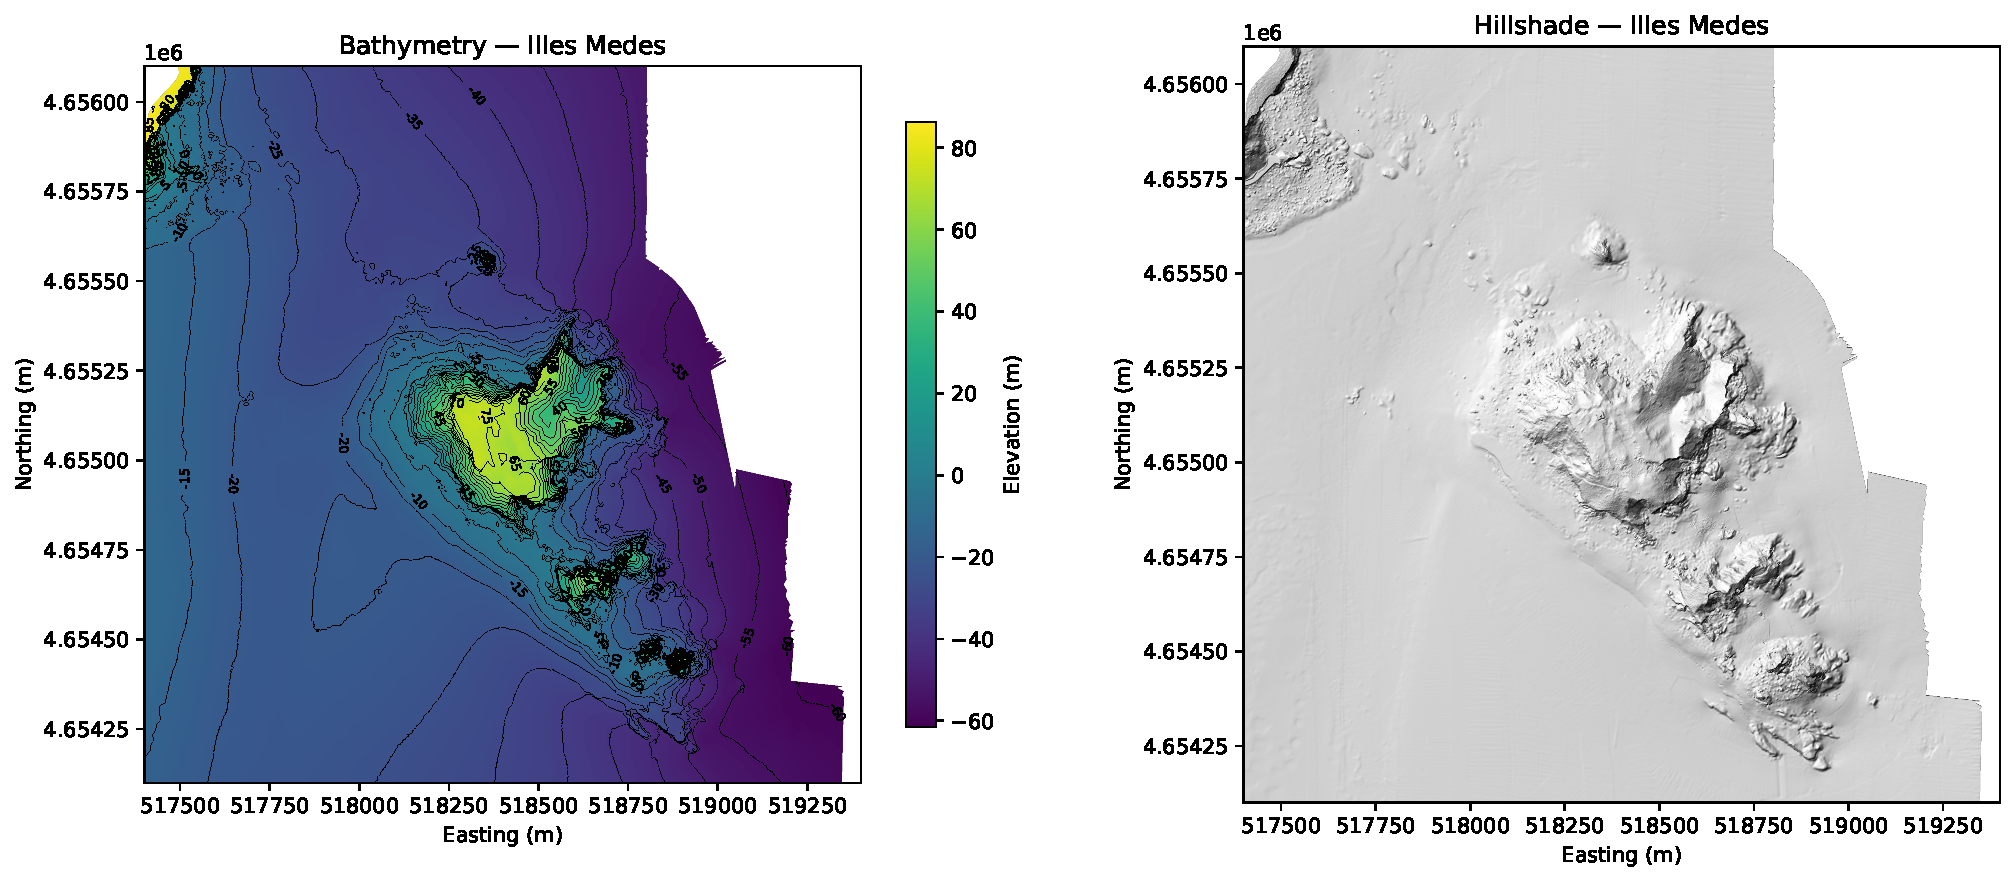
\includegraphics[width=\textwidth]{medes_bathymetry.pdf}
\caption{Illes Medes bathymetry. \textbf{Left:} Elevation with 5\,m contour intervals
(viridis colormap). \textbf{Right:} Analytical hillshade (azimuth 315\textdegree,
altitude 45\textdegree, vertical exaggeration 2$\times$). The Medes Islands are visible
as emerged outcrops in the northeast, with steep submarine walls descending to
\SI{-20}{m} to the west.}
\label{fig:bathymetry}
\end{figure}

%=============================================================================
\section{Terrain Morphometrics}
\label{sec:metrics}
%=============================================================================

Four terrain metrics were computed from the elevation grid, all at native 1\,m resolution.
NoData areas were handled by masking prior to computation and propagating NoData to output
cells where valid neighbors were insufficient.

\subsection{Slope}
\label{sec:slope}

Slope magnitude was computed from the first-order partial derivatives of the elevation
surface using central finite differences \citep{wilson2007}:

\begin{equation}
\text{slope} = \arctan\!\left(\sqrt{\left(\frac{\partial z}{\partial x}\right)^{\!2} +
\left(\frac{\partial z}{\partial y}\right)^{\!2}}\right)
\label{eq:slope}
\end{equation}

With the 1\,m grid spacing, $\partial z / \partial x$ and $\partial z / \partial y$ were
obtained via \texttt{numpy.gradient}:

\begin{lstlisting}
dz_dy, dz_dx = np.gradient(elevation, 1.0, 1.0)
slope_rad = np.arctan(np.sqrt(dz_dx**2 + dz_dy**2))
slope_deg = np.degrees(slope_rad)
\end{lstlisting}

The resulting slope ranges from 0\textdegree\ to 88.9\textdegree\ (mean
6.1\textdegree, $\sigma$ = 12.1\textdegree). The near-vertical maxima occur at the
cliff faces of the islands, which represent classic wall dive topography.

\subsection{Bathymetric Position Index (BPI)}
\label{sec:bpi}

The Bathymetric Position Index \citep{lundblad2006} quantifies whether a cell sits on a
local ridge (positive), in a depression (negative), or on a flat/slope (near zero):

\begin{equation}
\text{BPI} = z_{\text{cell}} - \overline{z}_{\text{annulus}}
\label{eq:bpi}
\end{equation}

where $\overline{z}_{\text{annulus}}$ is the mean elevation within an annular neighborhood
of inner radius $r_i$ and outer radius $r_o$. Two scales were computed:

\begin{itemize}
\item \textbf{Fine scale} ($r_i = 3$\,m, $r_o = 5$\,m): captures meter-scale features
such as individual boulders and small ridges.
\item \textbf{Broad scale} ($r_i = 25$\,m, $r_o = 50$\,m): captures the large-scale
terrain position---island platforms, inter-island channels, shelf breaks.
\end{itemize}

The annular mean was computed via 2D convolution with an explicit annular kernel, using a
separate validity mask convolution to correct for NoData at data boundaries:

\begin{lstlisting}
# Boolean annular kernel
y, x = np.ogrid[-r_o:r_o+1, -r_o:r_o+1]
annulus = ((np.sqrt(x**2 + y**2) >= r_i)
         & (np.sqrt(x**2 + y**2) <= r_o)).astype(float)

# NoData-aware convolution
elev_sum = ndimage.convolve(elev_filled, annulus, mode="constant")
valid_count = ndimage.convolve(valid_mask, annulus, mode="constant")
annular_mean = elev_sum / np.maximum(valid_count, 1.0)
bpi = elevation - annular_mean
\end{lstlisting}

Table~\ref{tab:bpi} summarizes the BPI statistics. The near-zero means confirm correct
implementation (BPI is a zero-mean statistic by construction over large areas). The
substantially larger spread at broad scale ($\sigma = 6.1$\,m vs.\ $1.1$\,m) indicates
that the dominant terrain structure at Illes Medes operates at the 25--50\,m scale,
consistent with the geomorphology of rocky island groups.

\begin{table}[ht]
\centering
\caption{BPI statistics at fine and broad scales.}
\label{tab:bpi}
\begin{tabular}{@{}lS[table-format=-2.3]S[table-format=2.3]S[table-format=-1.3]S[table-format=1.3]@{}}
\toprule
Scale & {Min (m)} & {Max (m)} & {Mean (m)} & {Std (m)} \\
\midrule
Fine ($r$ = 3--5\,m)   & -45.949 & 47.719 & 0.000 & 1.063 \\
Broad ($r$ = 25--50\,m) & -55.079 & 57.659 & 0.157 & 6.053 \\
\bottomrule
\end{tabular}
\end{table}

\subsection{Vector Ruggedness Measure (VRM)}
\label{sec:vrm}

The Vector Ruggedness Measure \citep{sappington2007} captures terrain heterogeneity
independently of slope magnitude. Each cell's surface orientation is expressed as a 3D
unit normal vector, and VRM measures the dispersion of these vectors within a moving
window:

\begin{equation}
\mathbf{n}_i = \begin{pmatrix}
    \sin(\text{slope}_i)\,\sin(\text{aspect}_i) \\
    \sin(\text{slope}_i)\,\cos(\text{aspect}_i) \\
    \cos(\text{slope}_i)
\end{pmatrix},
\qquad
\text{VRM} = 1 - \frac{\left|\sum_{i=1}^{n} \mathbf{n}_i\right|}{n}
\label{eq:vrm}
\end{equation}

A 3$\times$3 window ($n = 9$) was used. The component sums were computed efficiently
using \texttt{scipy.ndimage.uniform\_filter} (a separable $O(N)$ filter) multiplied by
$n$ to recover the sum from the mean:

\begin{lstlisting}
n = window_size ** 2
x_sum = ndimage.uniform_filter(x, size=window_size,
                               mode="constant") * n
y_sum = ndimage.uniform_filter(y, size=window_size,
                               mode="constant") * n
z_sum = ndimage.uniform_filter(z, size=window_size,
                               mode="constant") * n
resultant = np.sqrt(x_sum**2 + y_sum**2 + z_sum**2)
vrm = 1.0 - (resultant / n)
\end{lstlisting}

VRM ranges from 0 (perfectly flat) to 1 (maximally rugged). The observed range of 0 to
0.904 (mean 0.005, $\sigma$ = 0.027) indicates that the seafloor is overwhelmingly
smooth, with ruggedness concentrated at the island cliff edges. Values above 0.3 cluster
exclusively around the steep rocky perimeters---precisely the features that define
high-quality wall and cave dive sites.

\subsection{Multi-Panel Comparison}

Figure~\ref{fig:terrain} presents all five metrics at identical spatial extent for
comparison. The complementarity of the metrics is evident: slope highlights gradients,
BPI identifies relative position, and VRM isolates terrain heterogeneity.

\begin{figure}[ht]
\centering
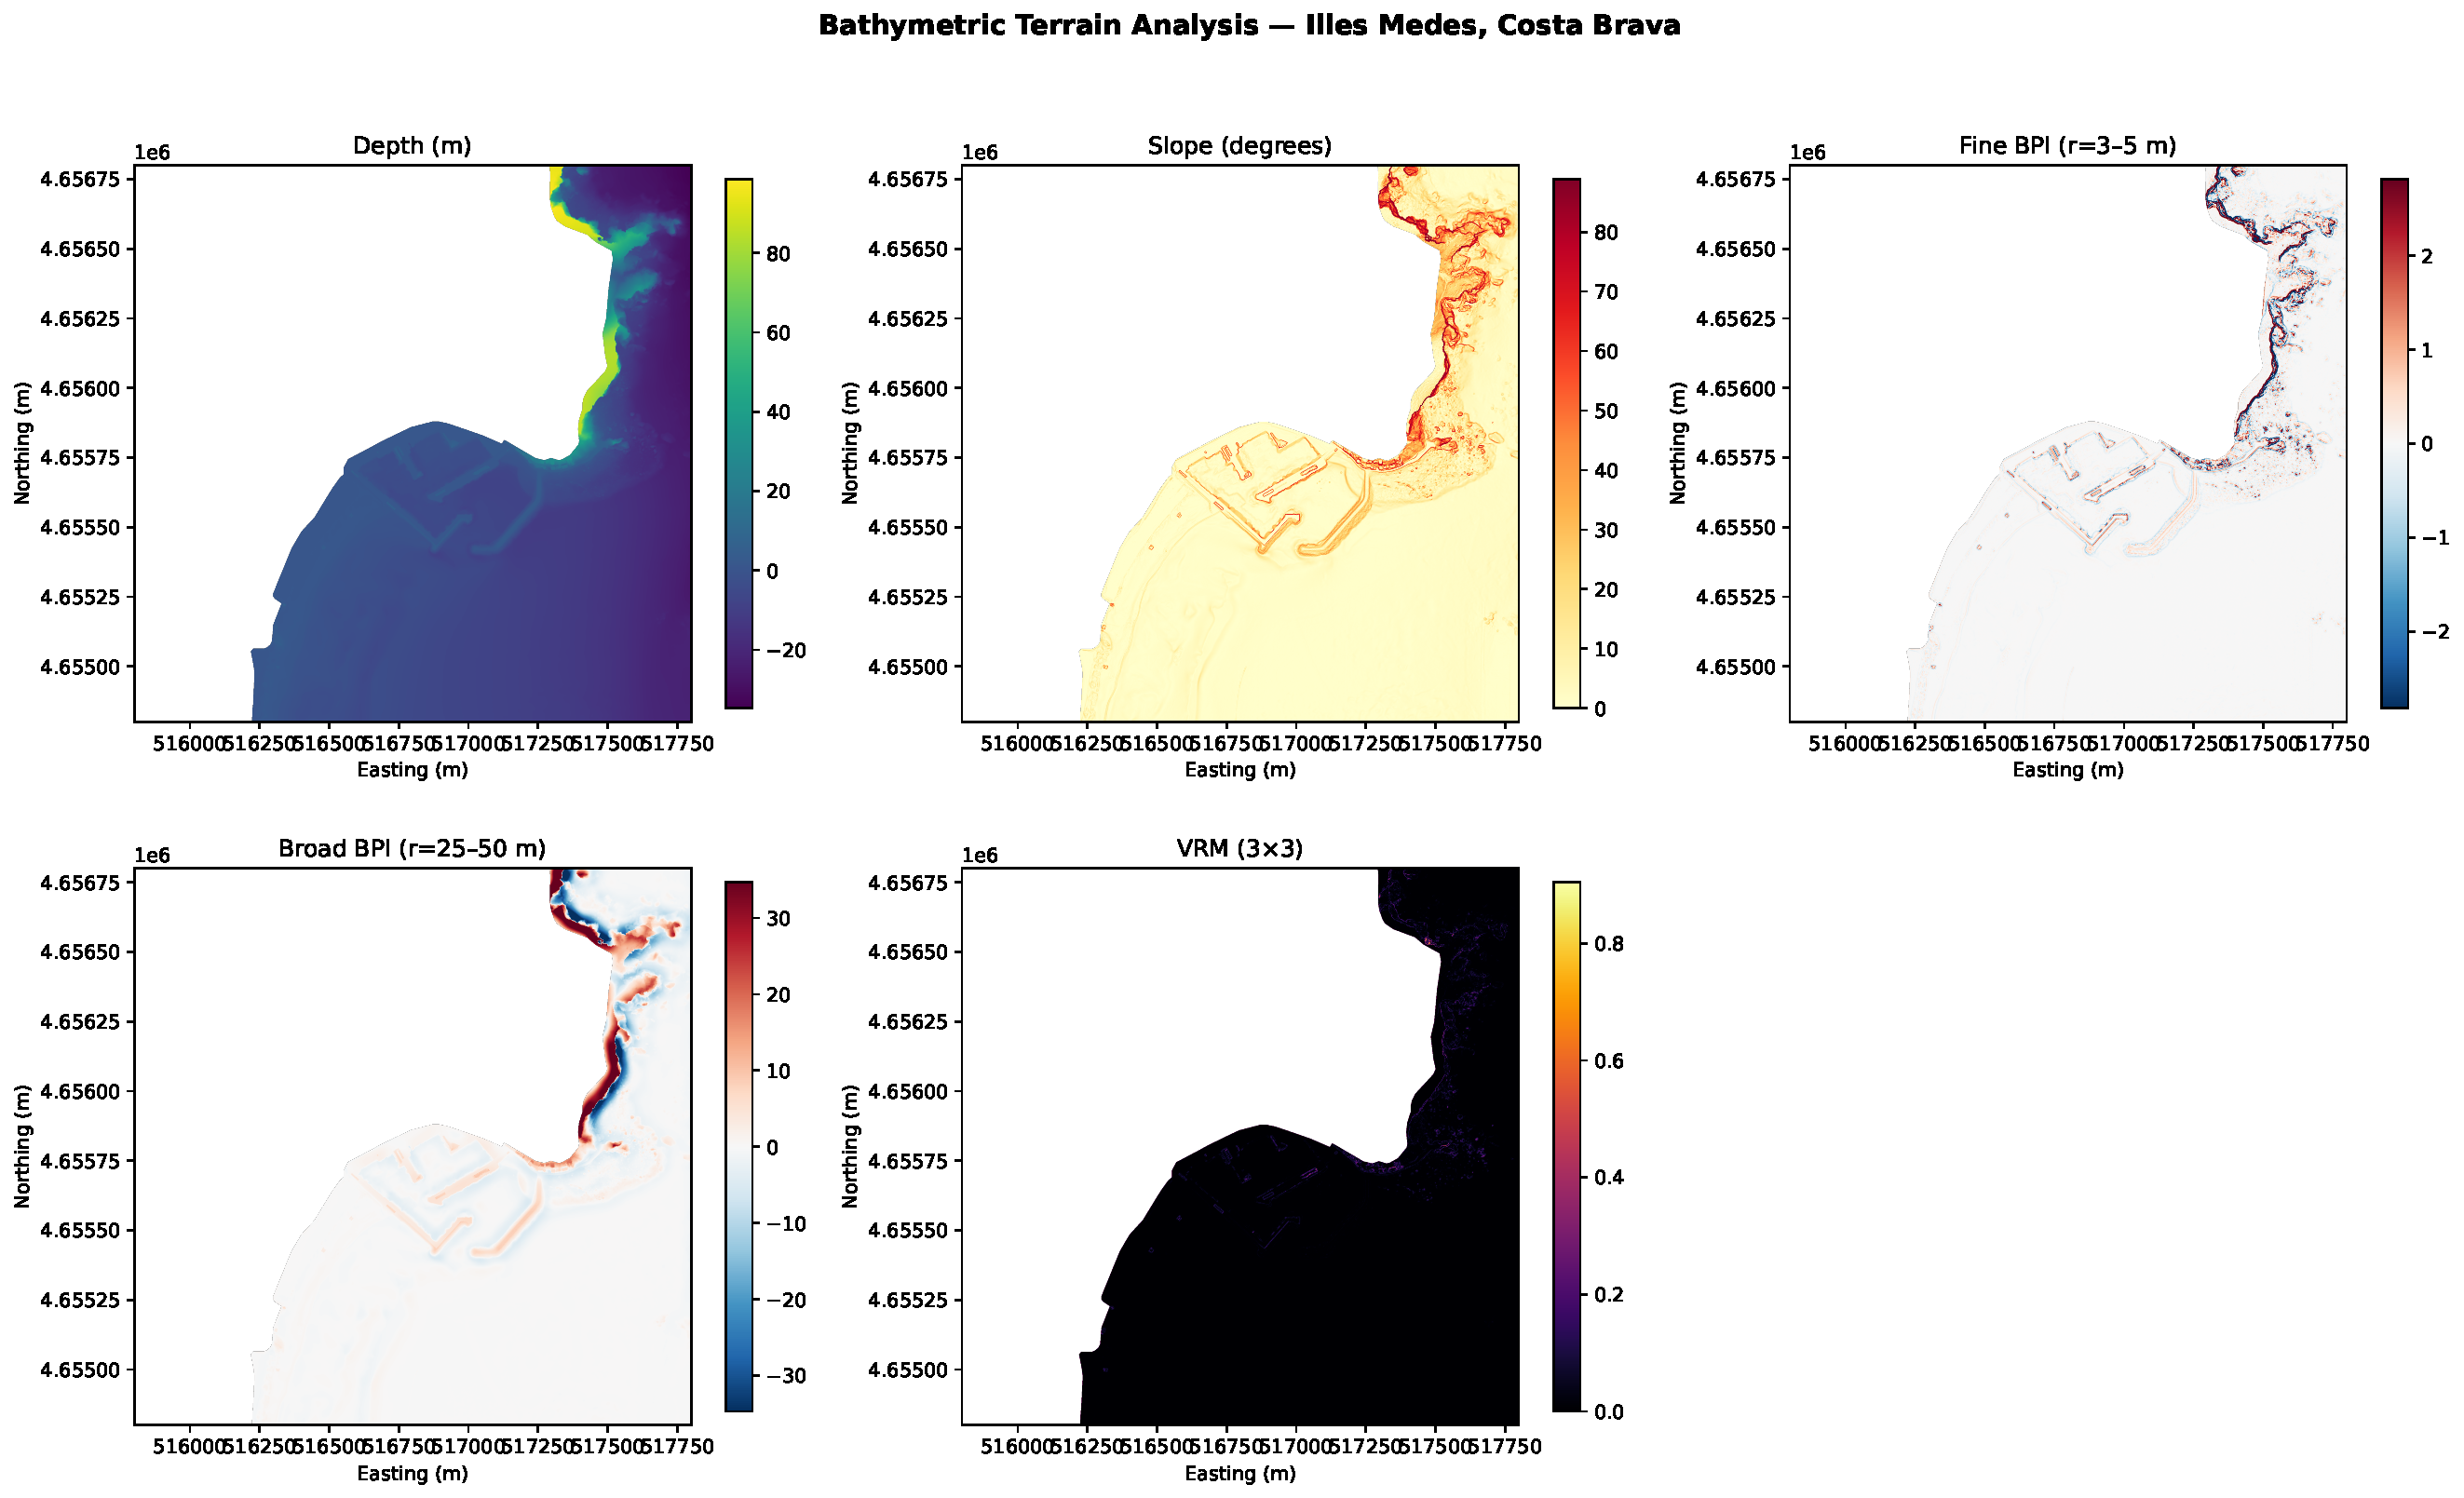
\includegraphics[width=\textwidth]{medes_terrain_analysis.pdf}
\caption{Bathymetric terrain analysis for Illes Medes. \textbf{Top row, left to right:}
depth (m), slope (degrees), fine-scale BPI ($r$ = 3--5\,m). \textbf{Bottom row:}
broad-scale BPI ($r$ = 25--50\,m), VRM (3$\times$3 window). BPI panels use a diverging
colormap centered at zero (red = ridges, blue = depressions).}
\label{fig:terrain}
\end{figure}

%=============================================================================
\section{Depth Profile Analysis}
\label{sec:profile}
%=============================================================================

An east--west transect at northing \SI{4655600}{m} was extracted across the study area
(Figure~\ref{fig:profile}). The profile reveals:

\begin{enumerate}
\item A shallow emerged platform (0--3\,m above sea level) corresponding to the island
    group, spanning approximately 500\,m horizontally.
\item A steep submarine wall descending from sea level to approximately \SI{-15}{m} over
    less than \SI{50}{m} of horizontal distance---a gradient exceeding 16\textdegree.
\item A gradual deepening to approximately \SI{-20}{m} over the remaining 500\,m eastward.
\end{enumerate}

Recreational diving certification thresholds are annotated: Open Water Diver (OWD,
\SI{12}{m}), Advanced Open Water Diver (AOWD, \SI{18}{m}), Deep Diver (\SI{30}{m}), and
the recreational limit (\SI{40}{m}). The Medes site reaches AOWD-accessible depths
within the survey extent, confirming its suitability for intermediate-level recreational
diving.

\begin{figure}[ht]
\centering
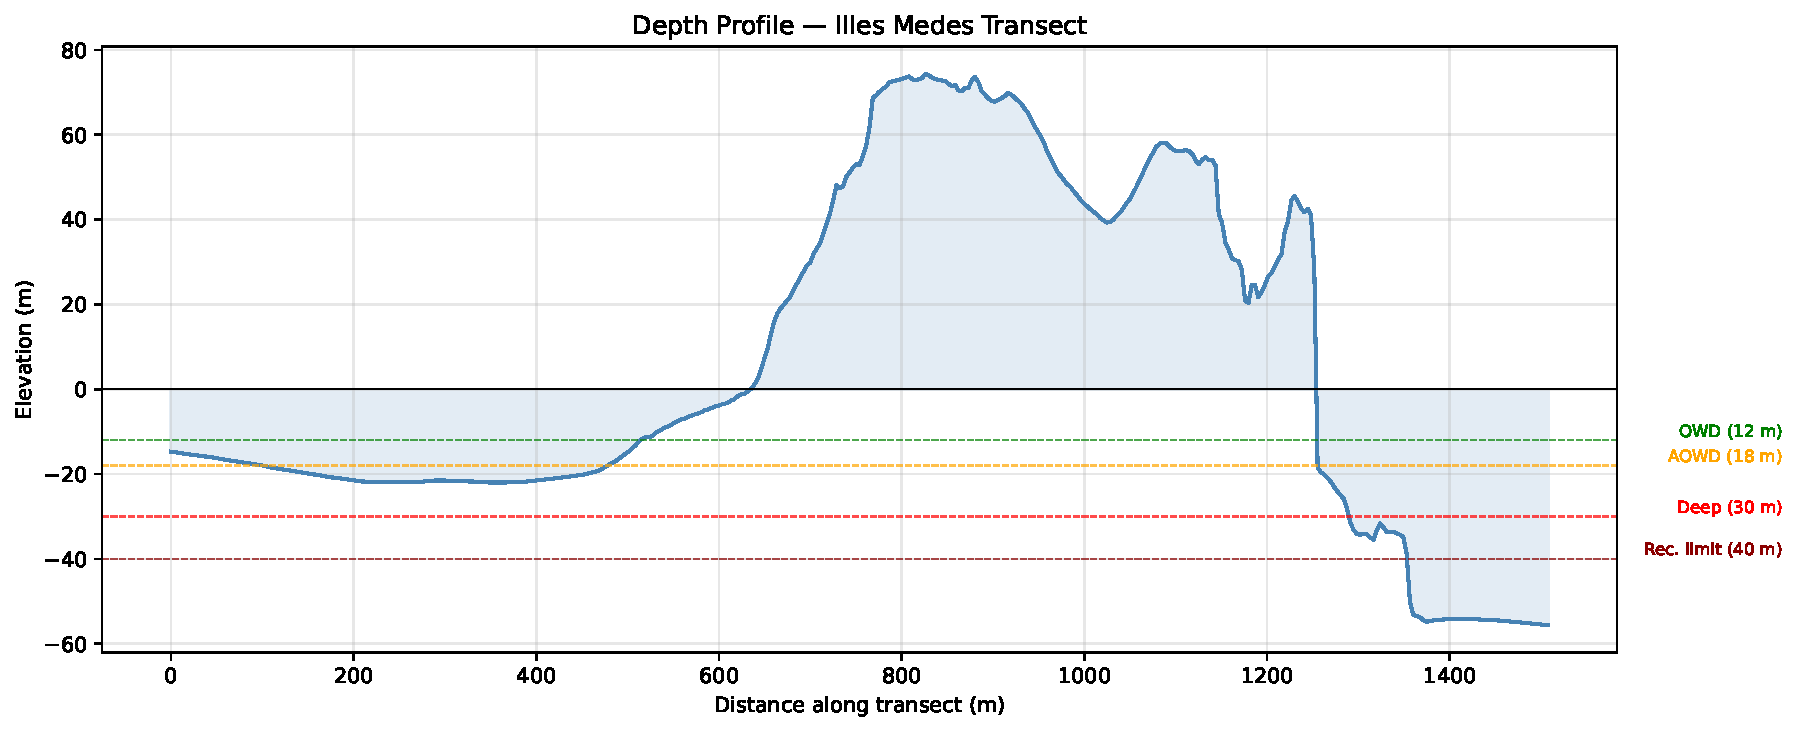
\includegraphics[width=\textwidth]{medes_depth_profile.pdf}
\caption{Depth profile along an E--W transect at $N$ = \SI{4655600}{m}. Dashed horizontal
lines indicate recreational diving certification depth limits. The steep wall feature
(\SI{0}{m} to \SI{-15}{m} over $\sim$\SI{50}{m} horizontal) is characteristic of the
island cliff morphology.}
\label{fig:profile}
\end{figure}

%=============================================================================
\section{Coast-Wide Analysis}
\label{sec:coast}
%=============================================================================

To assess the generalizability of the terrain metrics beyond the Illes Medes pilot area,
the analysis was extended to six sites spanning the full length of the Catalan coast
(approximately 240\,km). Sites were selected to represent a range of coastal
geomorphologies: rocky capes, island groups, and gently sloping continental shelf
(Figure~\ref{fig:coast_overview}).

\begin{figure}[ht]
\centering
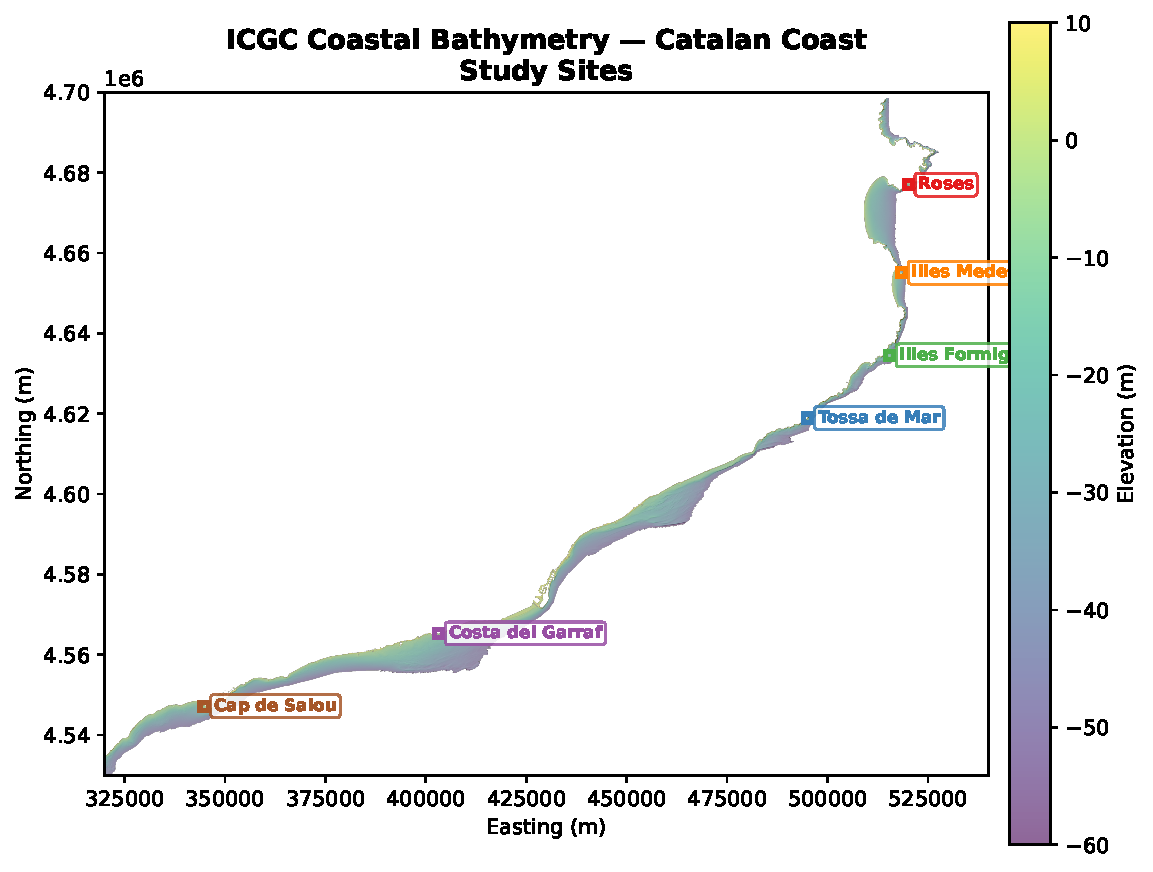
\includegraphics[width=0.75\textwidth]{coast_overview.pdf}
\caption{ICGC coastal bathymetry overview (64\,m resolution) with the six study sites
marked. The dataset covers a narrow littoral fringe from the French border (NE) to Cap
de Salou (SW). Background: hillshade with semi-transparent bathymetry overlay.}
\label{fig:coast_overview}
\end{figure}

\subsection{Site Selection}

Table~\ref{tab:sites} describes the six study areas. Each site was extracted as a
2\,km~$\times$~2\,km window at full 1\,m resolution from the remote COG, and all four
terrain metrics were computed identically.

\begin{table}[ht]
\centering
\caption{Study sites along the Catalan coast. Coordinates are window centers in
EPSG:25831.}
\label{tab:sites}
\begin{tabular}{@{}llrrl@{}}
\toprule
Site & Label & Easting & Northing & Character \\
\midrule
1 & Roses              & 520\,000 & 4\,686\,500 & Rocky cape, steep cliffs \\
2 & Illes Medes        & 516\,800 & 4\,655\,800 & Island MPA, walls \& tunnels \\
3 & Illes Formigues    & 515\,500 & 4\,636\,000 & Rocky islets, gentle shelf \\
4 & Tossa de Mar       & 494\,500 & 4\,619\,500 & Medieval coast, steep cliffs \\
5 & Costa del Garraf    & 406\,500 & 4\,565\,000 & Smooth continental shelf \\
6 & Cap de Salou       & 345\,500 & 4\,547\,500 & Rocky cape, moderate relief \\
\bottomrule
\end{tabular}
\end{table}

\subsection{Terrain Character Comparison}

Figure~\ref{fig:hillshades} shows the hillshade with depth overlay for each site,
revealing markedly different terrain character. Roses and Tossa de Mar display steep
coastal cliffs descending to $-$40--50\,m, while Costa del Garraf is a uniformly smooth
shelf with barely 20\,m of relief across the entire 2\,km window.

\begin{figure}[ht]
\centering
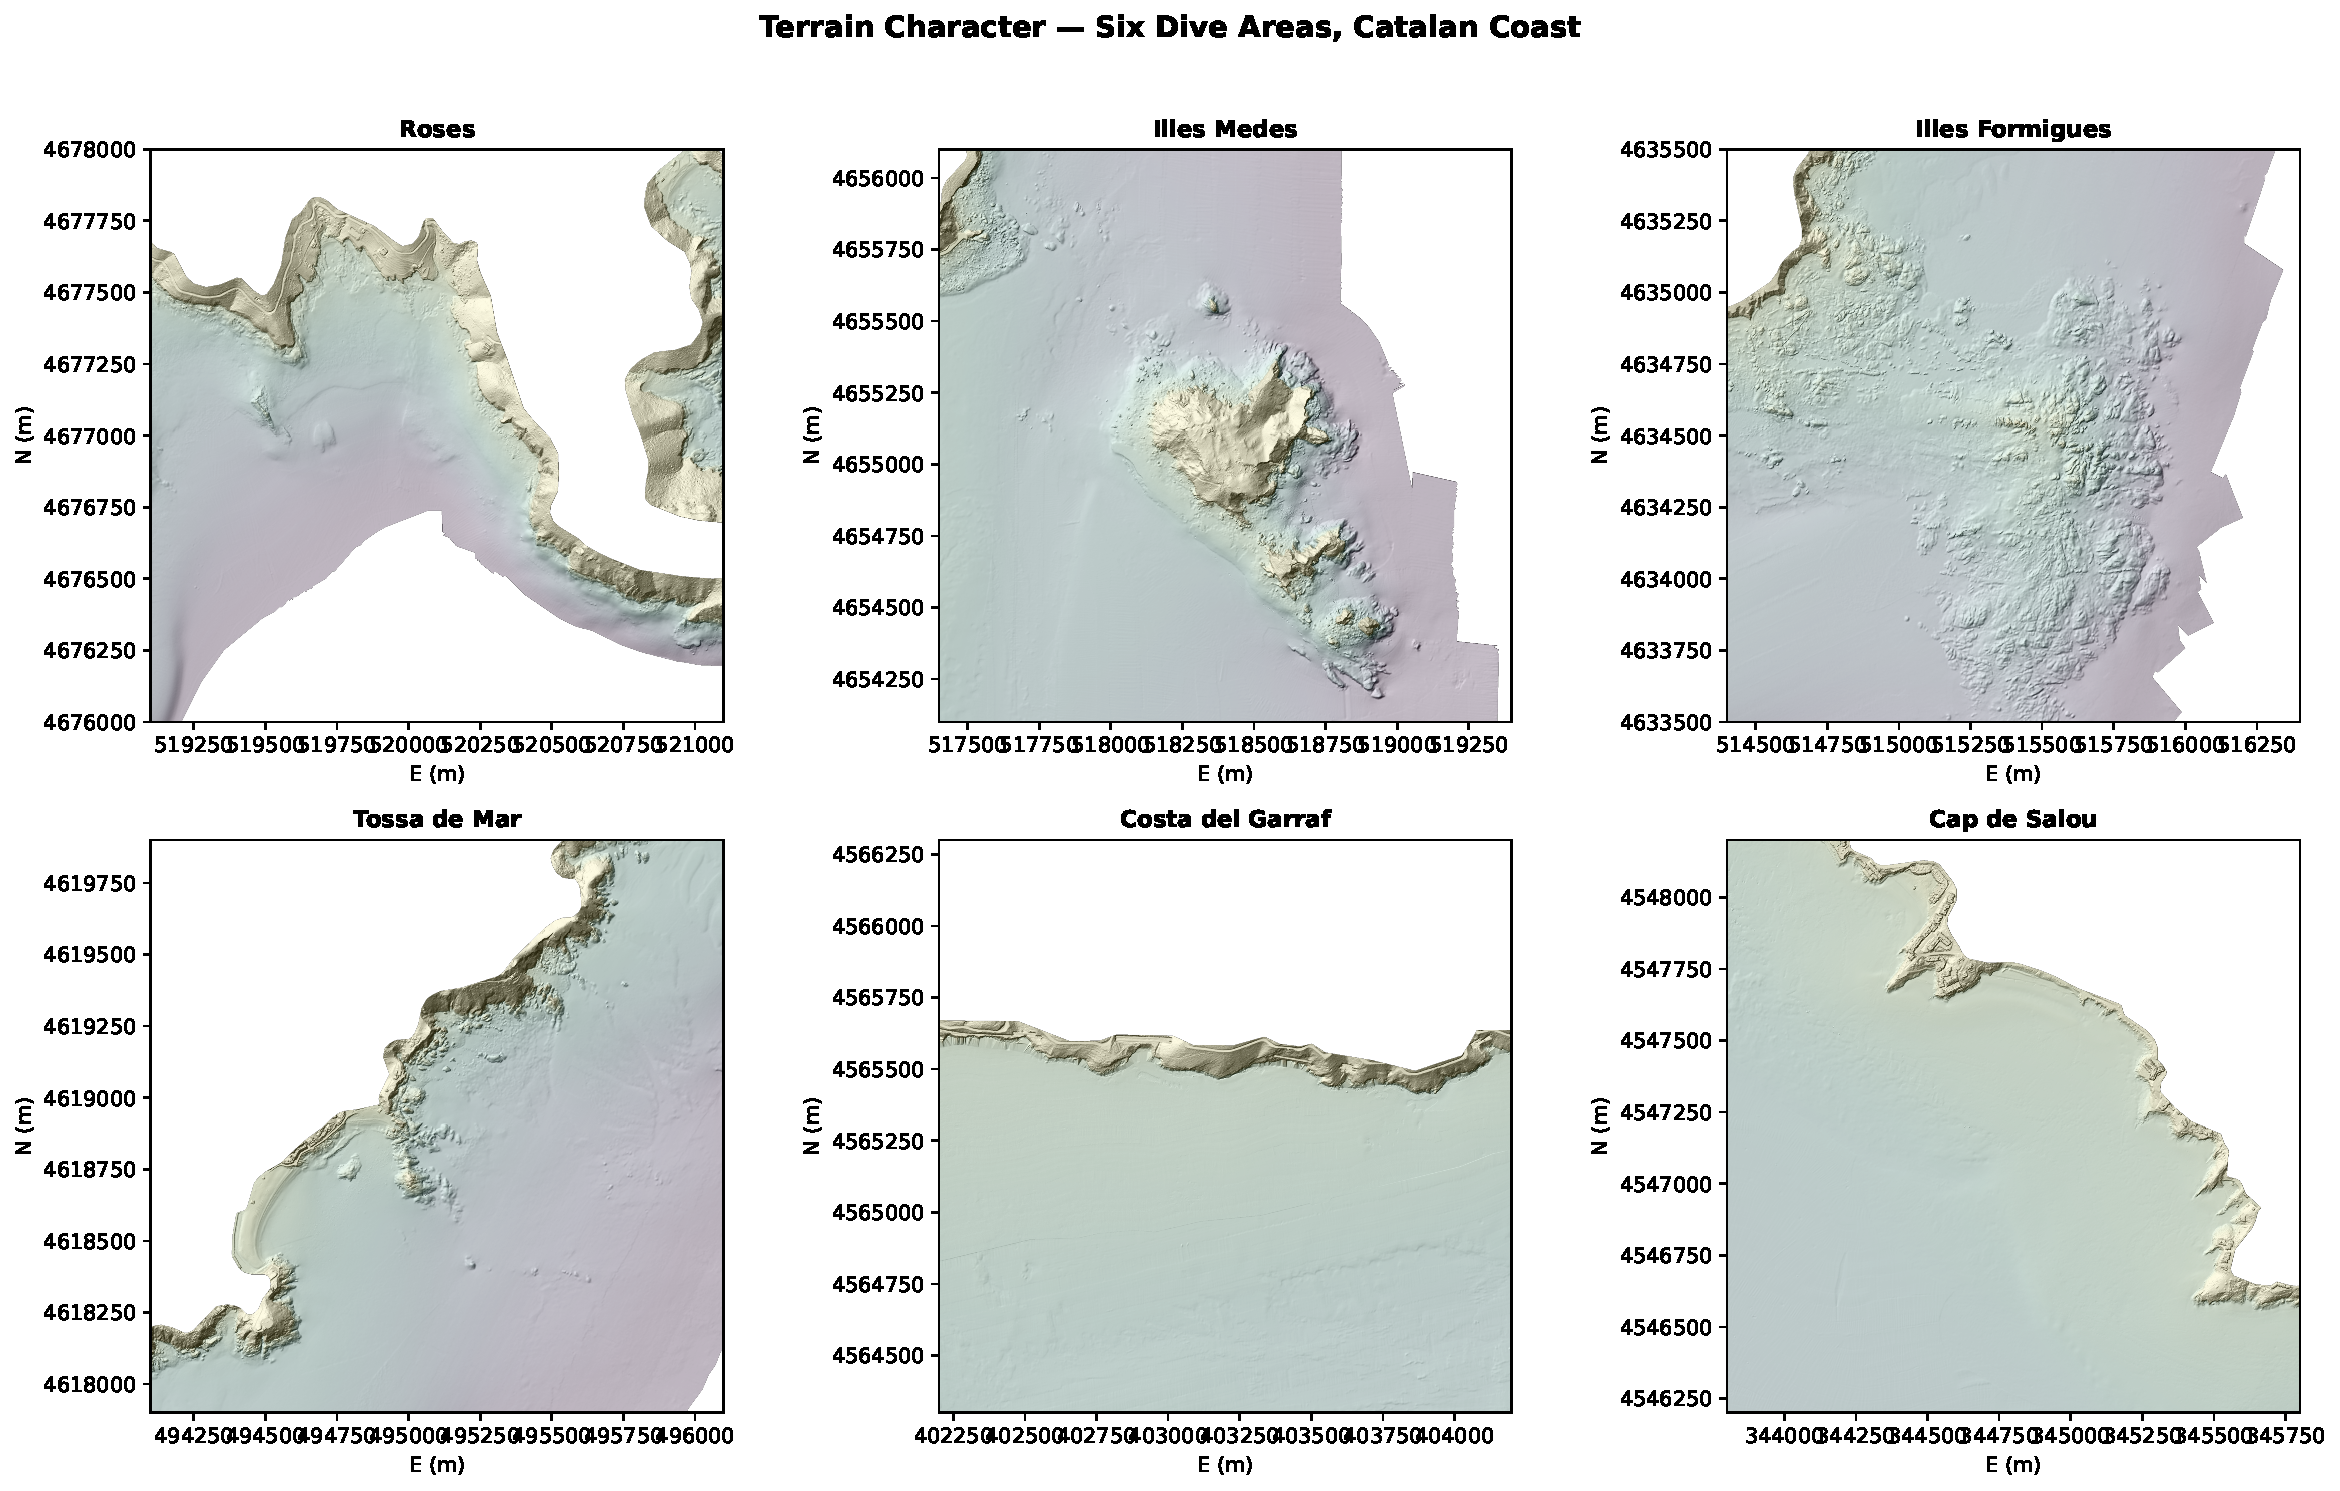
\includegraphics[width=\textwidth]{coast_site_hillshades.pdf}
\caption{Terrain character at six dive sites along the Catalan coast. Hillshade with
semi-transparent bathymetry overlay (viridis). Note the contrast between the steep,
rugged terrain at Roses and Tossa de Mar and the smooth shelf at Costa del Garraf.}
\label{fig:hillshades}
\end{figure}

\subsection{Comparative Statistics}

Table~\ref{tab:comparison} summarizes the terrain metrics across all sites.

\begin{table}[ht]
\centering
\caption{Comparative terrain metrics across the six study sites.}
\label{tab:comparison}
\begin{tabular}{@{}lS[table-format=2.1]S[table-format=2.1]S[table-format=1.4]S[table-format=1.2]@{}}
\toprule
Site & {Mean slope (\textdegree)} & {Max slope (\textdegree)} &
{Mean VRM} & {Broad BPI $\sigma$ (m)} \\
\midrule
Roses           & 16.1 & 89.0 & 0.0070 & 5.32 \\
Illes Medes     &  6.1 & 88.9 & 0.0050 & 6.05 \\
Illes Formigues &  5.1 & 87.0 & 0.0030 & 2.77 \\
Tossa de Mar    & 11.2 & 89.0 & 0.0080 & 5.32 \\
Costa del Garraf &  0.7 & 20.8 & 0.0010 & 0.10 \\
Cap de Salou    &  5.4 & 85.8 & 0.0070 & 3.34 \\
\bottomrule
\end{tabular}
\end{table}

Several patterns emerge:

\begin{enumerate}
\item \textbf{Roses and Tossa de Mar} are the steepest sites, with mean slopes of
    16.1\textdegree\ and 11.2\textdegree\ respectively, and the highest VRM values
    (0.007--0.008). Both are known for dramatic cliff-face diving.

\item \textbf{Costa del Garraf} stands in stark contrast: mean slope 0.7\textdegree,
    maximum slope only 20.8\textdegree, VRM effectively zero (0.001), and broad BPI
    $\sigma$ = 0.10\,m. This is a featureless sandy shelf---terrain metrics correctly
    identify it as having no geomorphological interest for dive site characterization.

\item \textbf{Broad BPI standard deviation} separates sites more cleanly than
    mean slope: Illes Medes has the highest $\sigma$ (6.05\,m) despite moderate mean
    slope, because the islands create strong positive anomalies surrounded by channels.
    This confirms that BPI captures terrain \emph{position} (ridges vs.\ depressions)
    independently of gradient magnitude.

\item \textbf{VRM is the most consistent discriminator} of ``interesting'' terrain.
    Sites known for quality diving (Roses, Medes, Tossa, Salou) all have
    VRM~$\geq$~0.005, while the featureless Garraf shelf scores 0.001.
\end{enumerate}

Figure~\ref{fig:boxplots} shows the full metric distributions as box plots, confirming
the statistical separation.

\begin{figure}[ht]
\centering
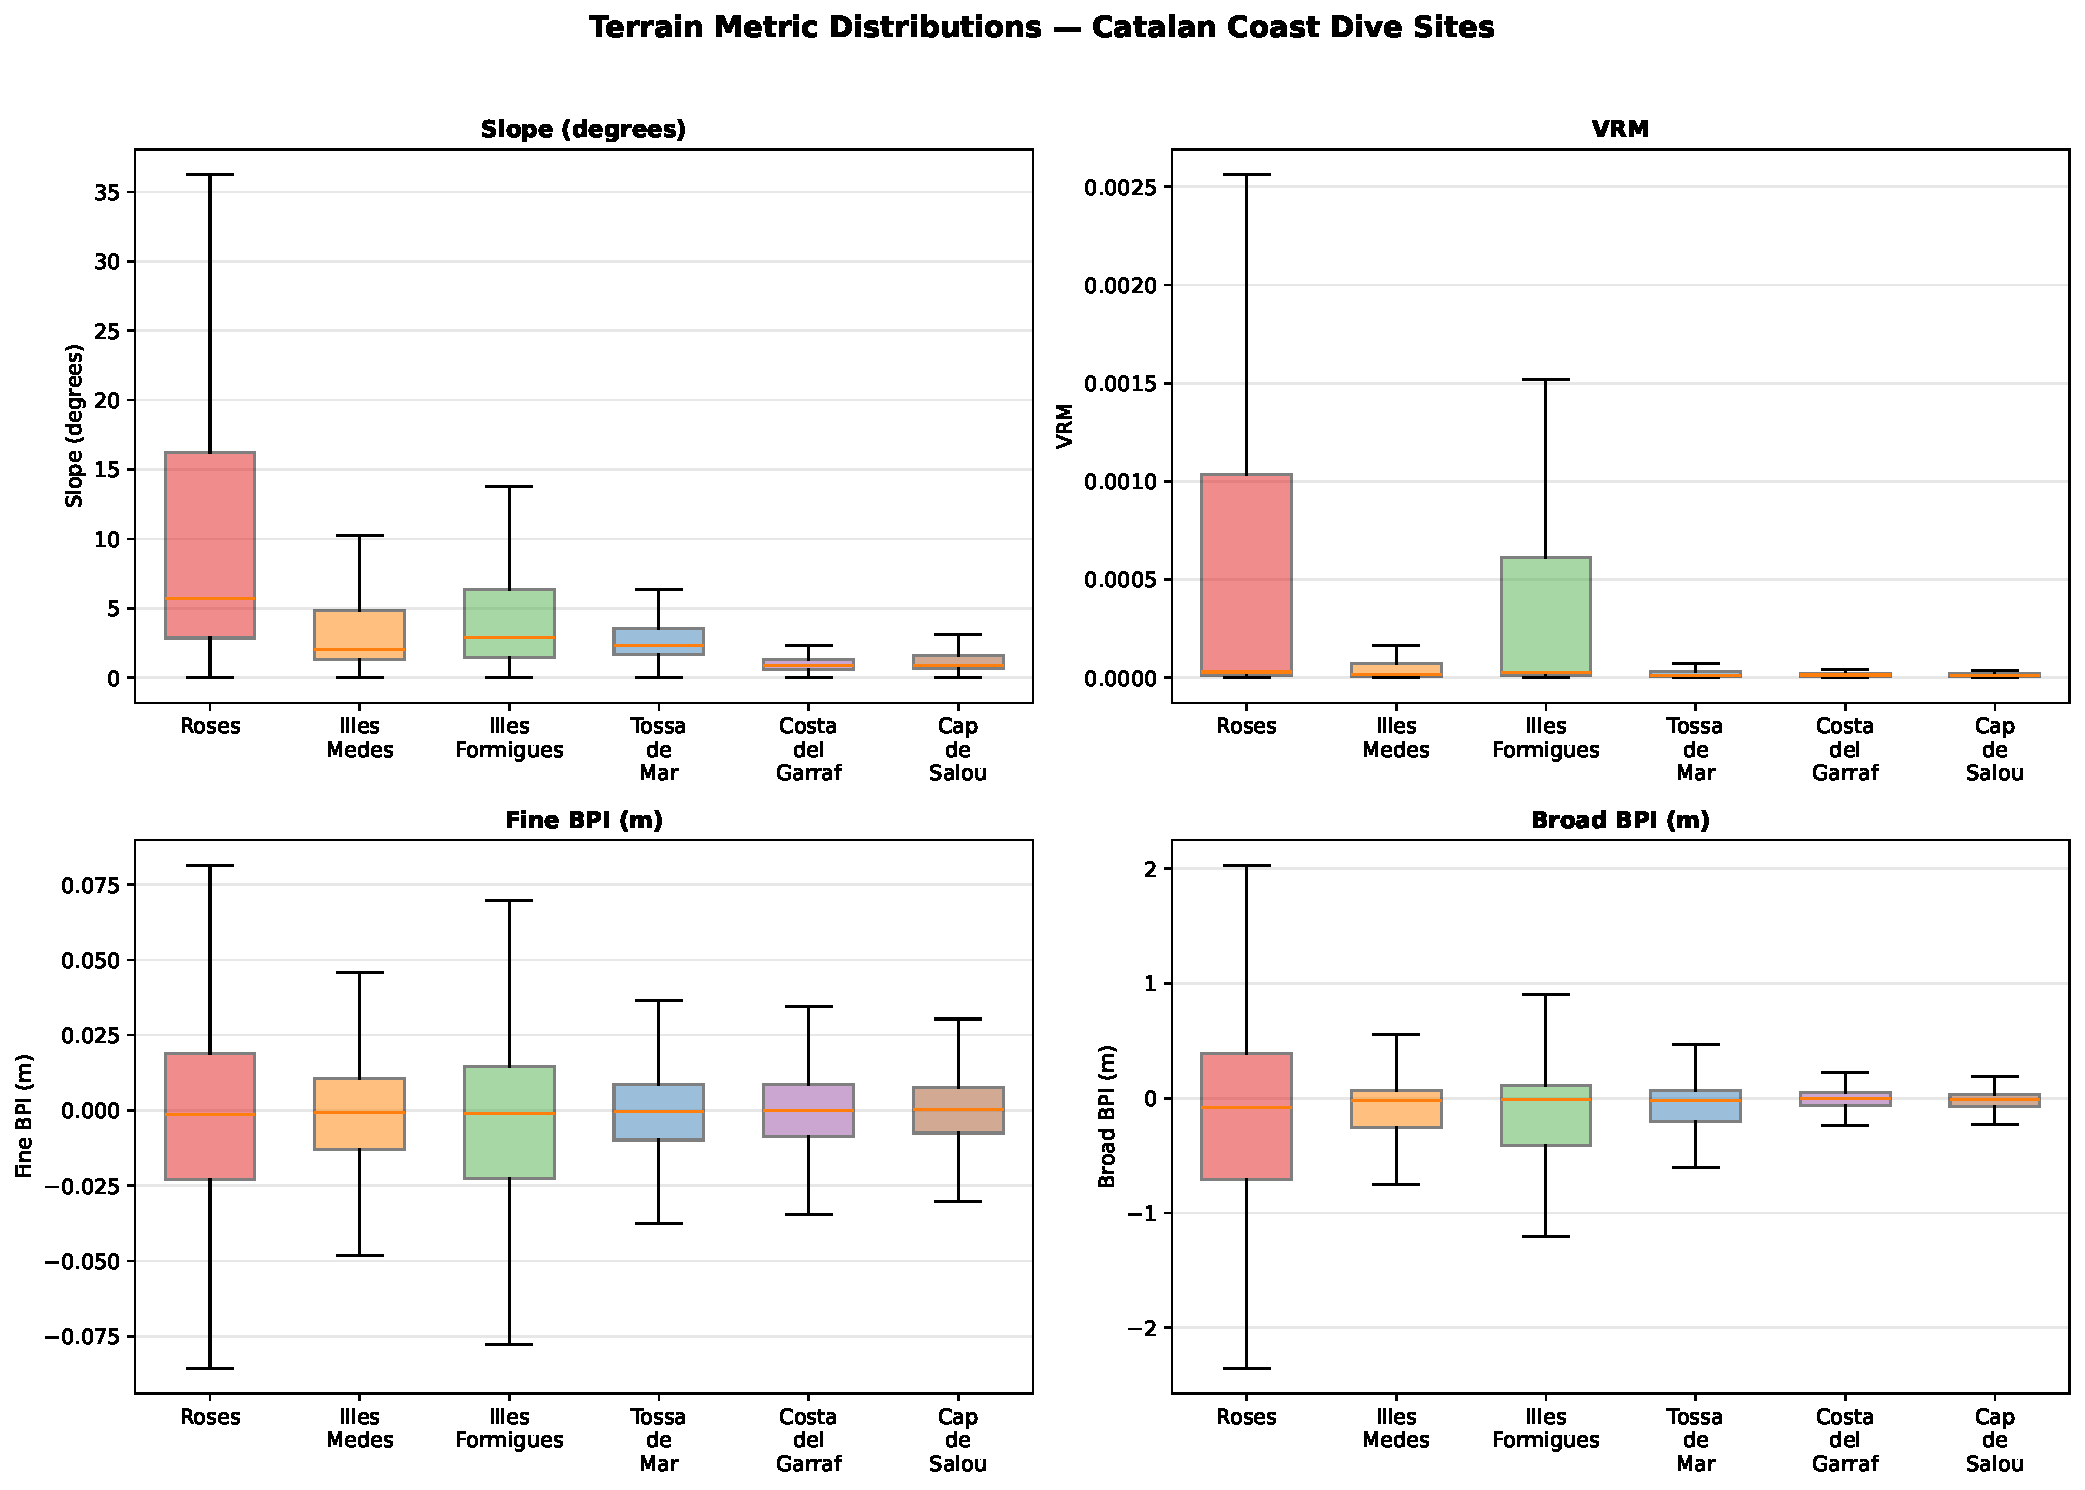
\includegraphics[width=\textwidth]{coast_metric_comparison.pdf}
\caption{Box plot comparison of terrain metric distributions across six Catalan coast
dive sites. Outliers suppressed for clarity. Roses and Tossa de Mar consistently show
the widest distributions (steepest, most variable terrain), while Costa del Garraf is
nearly uniform across all metrics.}
\label{fig:boxplots}
\end{figure}

%=============================================================================
\section{Case Study: El Biotop Artificial Reef}
\label{sec:biotop}
%=============================================================================

To test the dataset's ability to detect anthropogenic underwater structures, we examined
the location of El Biotop, an artificial reef near Torredembarra (Tarragona). El Biotop
is a conical pyramid constructed from approximately 40\,000 tonnes of calcium carbonate
rock, with its base at $-$34\,m and its peak at $-$12\,m depth---a 22\,m vertical
structure. Completed in 2023, it has become the only known cleaning station for ocean
sunfish (\emph{Mola mola}) in Catalonia, making it a significant dive destination.

\subsection{Analysis}

The reported coordinates (41.130\textdegree\,N, 1.430\textdegree\,E; UTM:
368\,222\,E, 4\,554\,372\,N) were converted to EPSG:25831 and a
500\,m~$\times$~500\,m window was extracted at full 1\,m resolution
(Figure~\ref{fig:biotop}). All four terrain metrics were computed.

The results show a uniformly smooth, gently sloping seafloor at approximately $-$39\,m
depth: mean slope 1.0\textdegree, VRM effectively zero ($10^{-5}$), and no BPI
anomaly. A wider 2\,km scan searching for local depth anomalies (cell elevation minus
100\,m neighborhood mean) found a maximum positive anomaly of only +2.1\,m, located
900\,m from the reported coordinates---far below the expected +22\,m signature of the
pyramid.

\begin{figure}[ht]
\centering
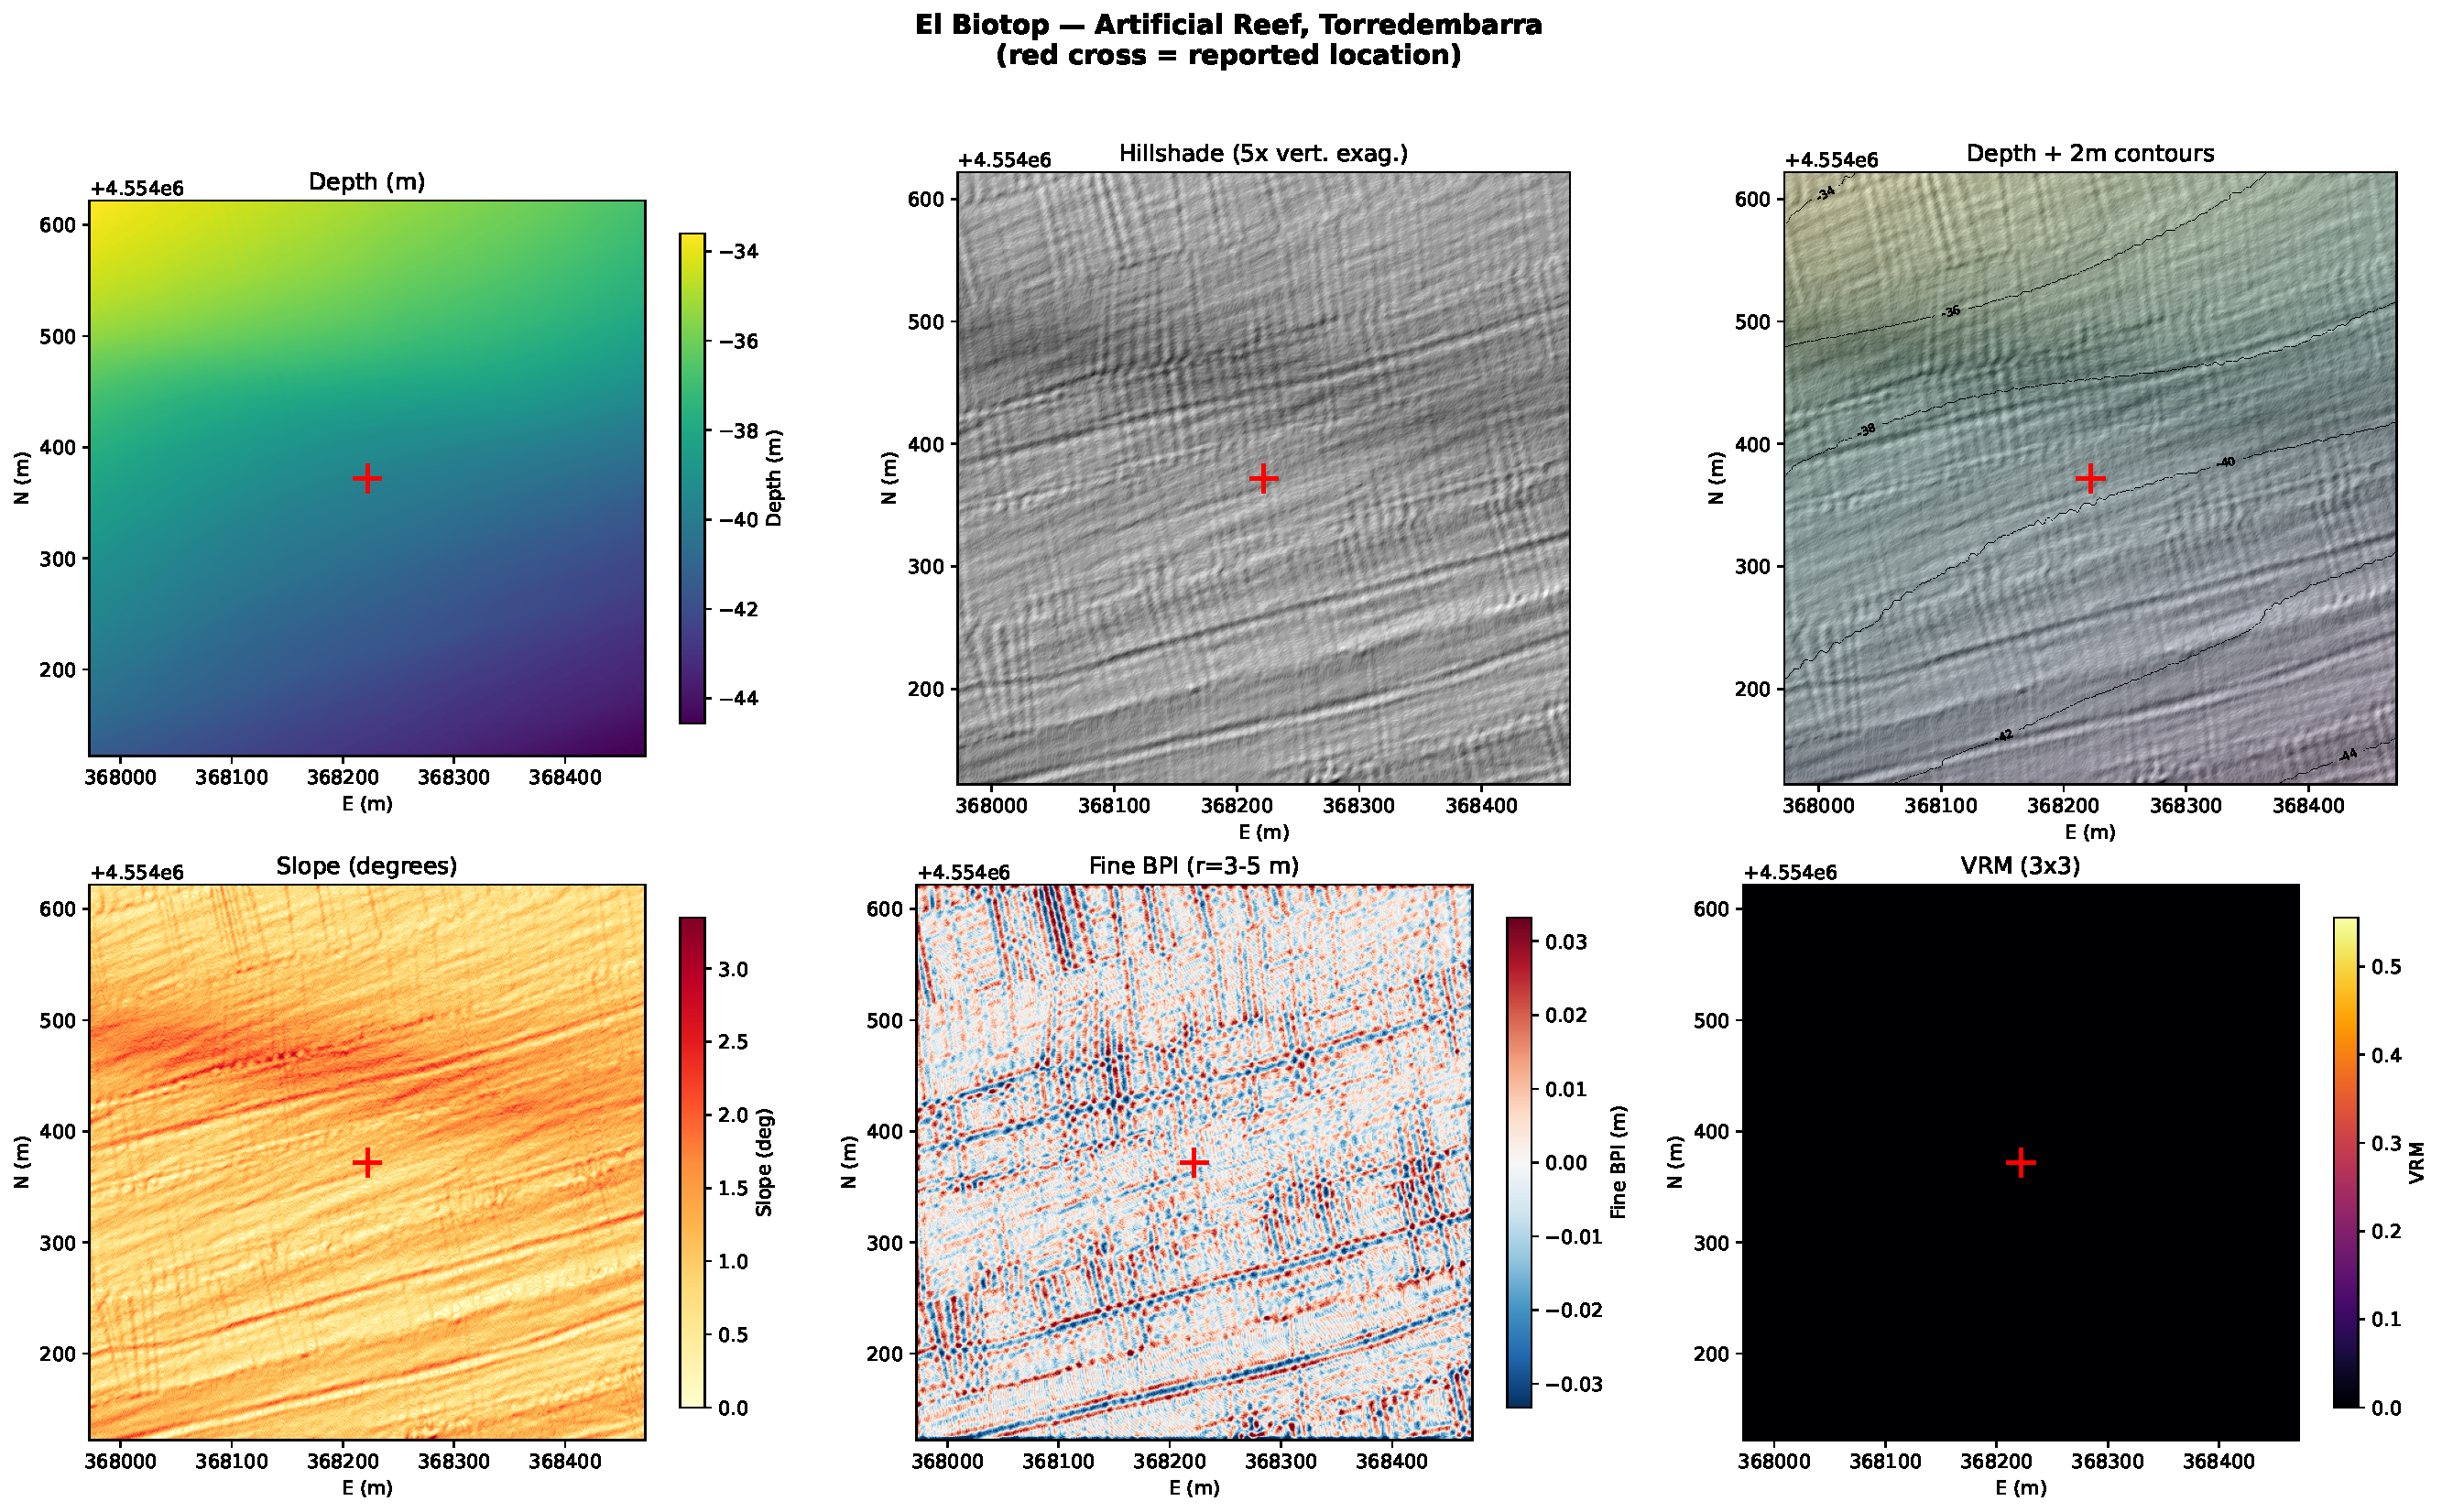
\includegraphics[width=\textwidth]{biotop_analysis.pdf}
\caption{Terrain analysis at the reported location of El Biotop artificial reef,
Torredembarra. \textbf{Top row:} depth, hillshade (5$\times$ vertical exaggeration),
depth with 2\,m contours. \textbf{Bottom row:} slope, fine BPI, VRM. The red cross
marks the reported position. No structure is visible; the seafloor is uniformly
smooth. Diagonal striping in the BPI panel reveals multibeam sonar survey-line
artifacts.}
\label{fig:biotop}
\end{figure}

\subsection{Interpretation}

The 22\,m-tall Biotop pyramid is absent from the ICGC bathymetry despite being well
within the survey's spatial and depth coverage. The most likely explanation is
\textbf{temporal}: the dataset version label ``v2r1-2021-2025'' refers to the product
release, not the acquisition date for each swath. The Torredembarra area was almost
certainly surveyed before the reef's 2023 completion.

This finding reveals an important limitation for SotaMar: the ICGC bathymetry is a
\textbf{static snapshot} whose acquisition dates vary by location along the coast.
Artificial reefs, recent coastal works, and other anthropogenic changes will not appear
unless the area has been resurveyed after installation. Two secondary observations are
also noteworthy:

\begin{itemize}
\item The diagonal striping visible in the fine BPI panel (Figure~\ref{fig:biotop},
    bottom center) is a characteristic artifact of hull-mounted multibeam echosounder
    (MBES) surveys, caused by systematic depth offsets between adjacent swath lines.
    These artifacts are typically sub-meter in amplitude but become visible in
    high-sensitivity derivative metrics like BPI.

\item The seafloor depth at the reported location ($-$39\,m) is broadly consistent with
    the Biotop's documented base depth of $-$34\,m, suggesting the coordinates are
    approximately correct but that the pre-construction seabed was slightly deeper than
    the design specification, or the coordinates refer to a nearby point.
\end{itemize}

%=============================================================================
\section{Discussion and Conclusions}
\label{sec:conclusions}
%=============================================================================

This exploration validates the ICGC bathymetric dataset as an excellent foundation for
the SotaMar dive site characterization system, both at the individual site level (Illes
Medes pilot) and across the full Catalan coast, while also identifying critical temporal
limitations through the Biotop case study. Key findings:

\begin{enumerate}
\item \textbf{Data quality and access.} The 1\,m resolution captures dive-relevant
    features (walls, pinnacles, channels) at sub-meter vertical precision. The COG format
    enables efficient remote subsetting without downloading the 3.3\,GB file, making it
    practical to analyze arbitrary coastal windows on demand. Six 2\,km~$\times$~2\,km
    windows were extracted and analyzed in under four minutes of computation time.

\item \textbf{Metric complementarity.} No single metric fully characterizes dive site
    terrain. Slope identifies steep walls. Broad-scale BPI distinguishes ridges from
    channels. VRM isolates terrain heterogeneity. The coast-wide comparison demonstrates
    that these metrics are complementary: Illes Medes scores highest on BPI
    variability but only moderate on slope, while Roses leads on slope but not BPI.

\item \textbf{VRM as a dive site discriminator.} Across all six sites, VRM proved the
    most consistent single metric for separating sites with known dive interest from
    featureless terrain. A threshold of VRM~$>$~0.003 correctly separates the five
    geomorphologically interesting sites from the Garraf shelf.

\item \textbf{Scale sensitivity.} Fine-scale BPI ($r$ = 3--5\,m) shows minimal variation
    at all sites, confirming that dive-relevant terrain structure operates at scales of
    25--50\,m. Terrain classification should prioritize the broad-scale BPI.

\item \textbf{Temporal limitations.} The Biotop case study demonstrates that the ICGC
    bathymetry is a static snapshot with spatially variable acquisition dates. Artificial
    reefs and recent coastal modifications will not appear unless the area has been
    resurveyed. SotaMar must therefore treat the ICGC data as a \emph{baseline terrain
    layer} and maintain a separate registry of known artificial structures and recent
    changes, cross-referenced by installation date and survey vintage.

\item \textbf{Coverage limitations.} The ICGC survey covers only the littoral fringe to
    approximately $-$50\,m depth. Northern sites (Roses) have sparser coverage than
    central Costa Brava sites (Formigues: 82\% valid). Any automated pipeline must handle
    variable NoData density across the coast.
\end{enumerate}

The next step is to implement a terrain classification scheme based on combined BPI and
slope thresholds following the Benthic Terrain Modeler methodology
\citep{lundblad2006}, and to systematically score the full coastline for dive site
potential using the VRM-based discriminator identified here. The Biotop case also
motivates integrating temporal metadata (survey acquisition dates per swath) into the
SotaMar pipeline to flag areas where the bathymetry may be outdated.

%=============================================================================
% References
%=============================================================================

\begingroup
\renewcommand{\section}[2]{}  % suppress natbib section heading
\begin{thebibliography}{9}

\bibitem[Lloret et~al.(2008)]{lloret2008}
J.~Lloret, A.~Zaragoza, D.~Caballero, and V.~Riera.
\newblock Impacts of recreational boating on the marine environment of the Medes Islands,
Mediterranean Sea.
\newblock \emph{Ocean \& Coastal Management}, 51(11):749--754, 2008.

\bibitem[Lundblad et~al.(2006)]{lundblad2006}
E.~R. Lundblad, D.~J. Wright, J.~Miller, E.~M. Larkin, R.~Rinehart, D.~F. Naar,
B.~T. Donahue, S.~M. Anderson, and T.~Battista.
\newblock A benthic terrain classification scheme for American Samoa.
\newblock \emph{Marine Geodesy}, 29(2):89--111, 2006.

\bibitem[Sappington et~al.(2007)]{sappington2007}
J.~M. Sappington, K.~M. Longshore, and D.~B. Thompson.
\newblock Quantifying landscape ruggedness for animal habitat analysis: A case study
using bighorn sheep in the Mojave Desert.
\newblock \emph{Journal of Wildlife Management}, 71(5):1419--1426, 2007.

\bibitem[Wilson et~al.(2007)]{wilson2007}
M.~F.~J. Wilson, B.~O'Connell, C.~Brown, J.~C. Guinan, and A.~J. Grehan.
\newblock Multiscale terrain analysis of multibeam bathymetry data for habitat mapping
on the continental slope.
\newblock \emph{Marine Geodesy}, 30(1-2):3--35, 2007.

\end{thebibliography}
\endgroup

\end{document}
